\newpage
\section{CFD Model}

\subsection{Simulation parameters}
\label{subsec:simulation_parameters}

\subsubsection{Solver settings}

The simulations were performed with SolidWorks Flow Simulation, using an implicit finite‐volume solver. We employed the commercial CFD NIKA solver developed by Dassault Systèmes. It solves the three‐dimensional Navier–Stokes equations for a perfect gas, including a \(k\text{–}\varepsilon\) turbulence model and conjugate heat transfer (CHT).

\subsubsection{Geometry}

The flow over the slope depends only on two parameters: the slope angle \(\theta\) and the Mach number \(M\). Hence the shock angle is a function
\[
    \beta = f(\theta, M).
\]
\begin{figure}[H]
    \centering
    \begin{minipage}[b]{0.45\linewidth}
        \centering
        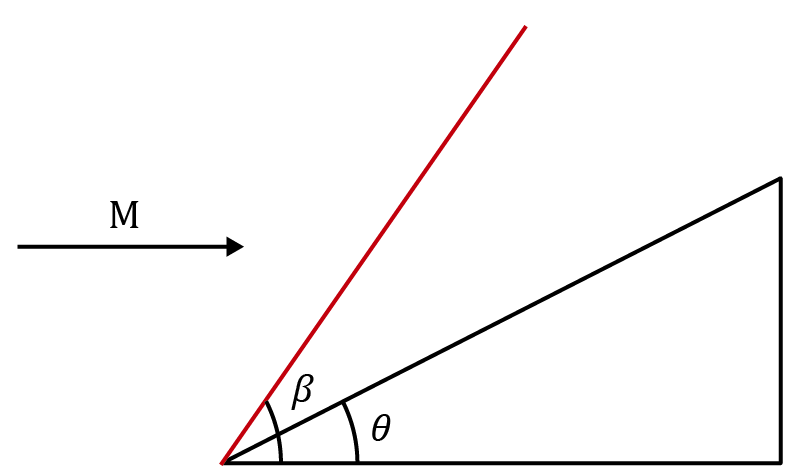
\includegraphics[width=\linewidth]{ressources/images/Slope.png}
        \caption{Slope geometry}
    \end{minipage}
    \hfill
    \begin{minipage}[b]{0.45\linewidth}
        \centering
        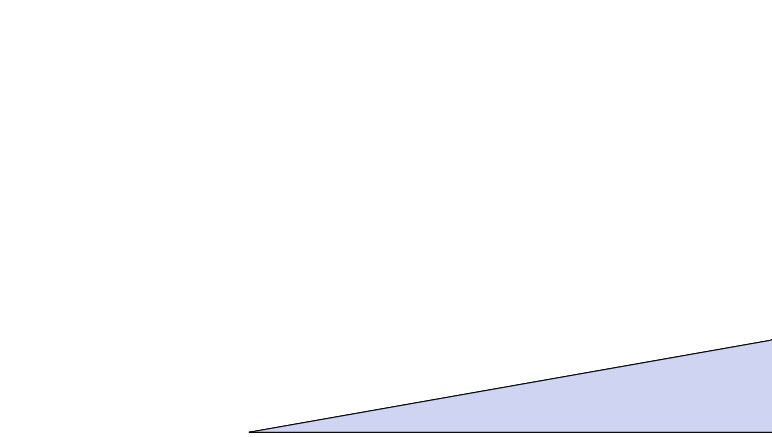
\includegraphics[width=\linewidth]{ressources/images/SlopeSW.jpg}
        \caption{SolidWorks model}
    \end{minipage}
    \label{fig:slope}
\end{figure}
The fixed geometric parameter is the triangle length, set to 50 cm.

\subsubsection{Mesh}

We use a two‐dimensional mesh with logarithmically varying refinement. In the coarsest region, the grid spacing is 0.0881 cm; in the finest region, it is 0.0042 cm.
\begin{figure}[H]
    \centering
    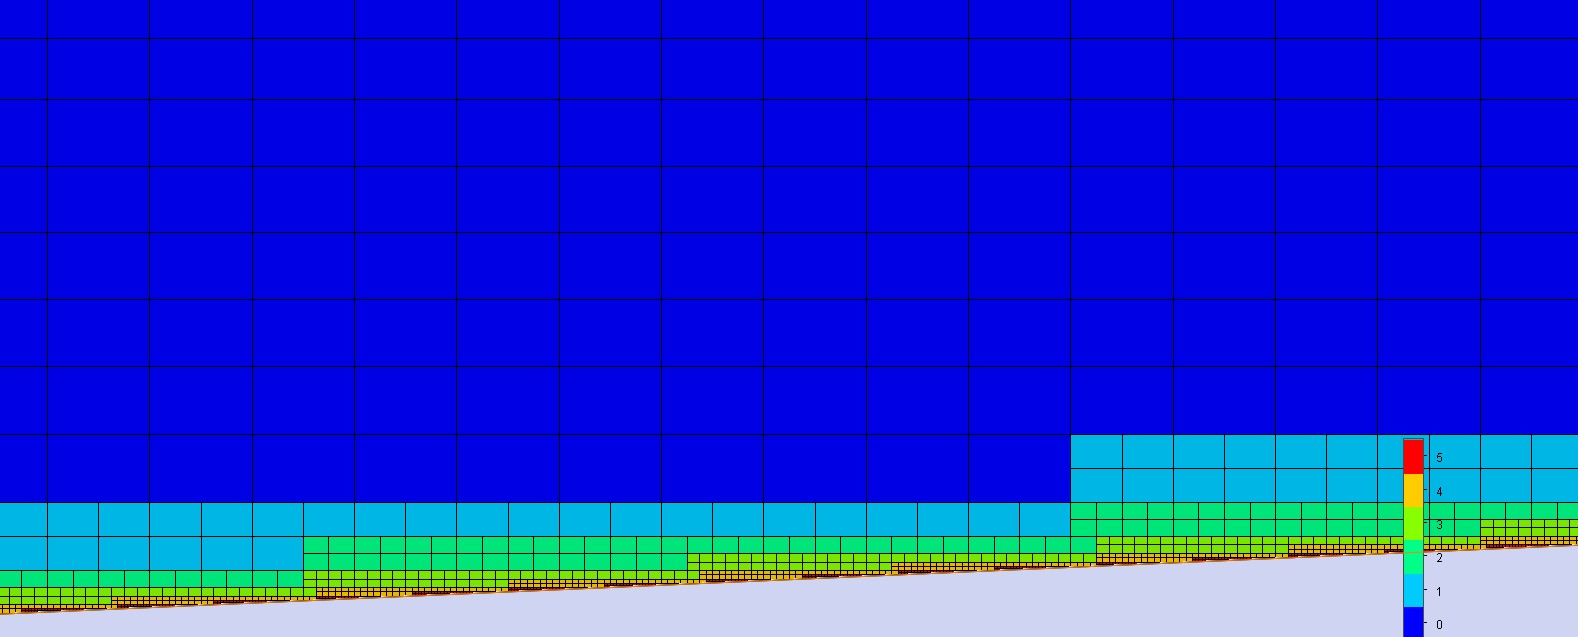
\includegraphics[width=0.8\linewidth]{ressources/images/CFD/Maillage.jpg}
    \caption{Computational mesh}
    \label{fig:mesh}
\end{figure}

\subsection{Simulation}

\subsubsection{Results}

To determine the shock angle \(\beta\), we compute the pressure at every point. The shock wave is located by identifying the pressure‐drop line, and its angle is measured relative to the \(x\)-axis. The simulation is run until the flow field converges.

\begin{figure}[H]
    \centering
    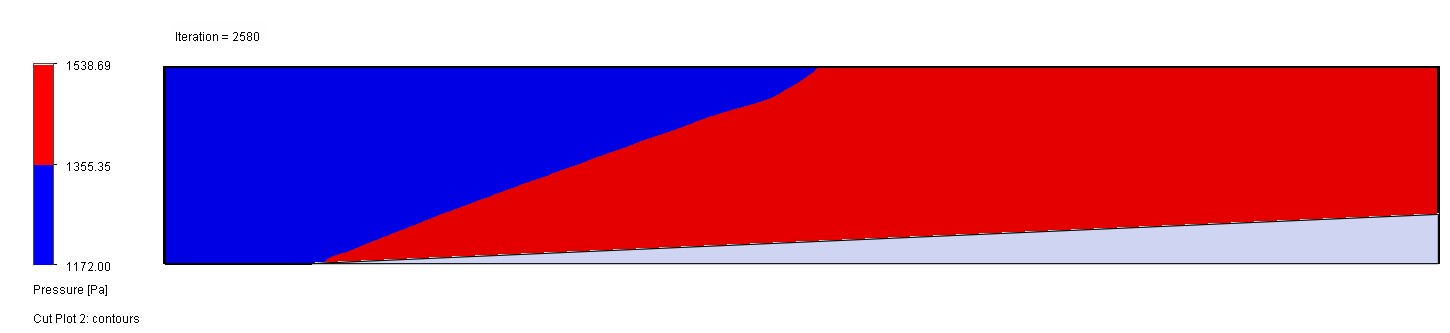
\includegraphics[width=0.8\linewidth]{ressources/images/CFD/SolidWorks1.jpg}
    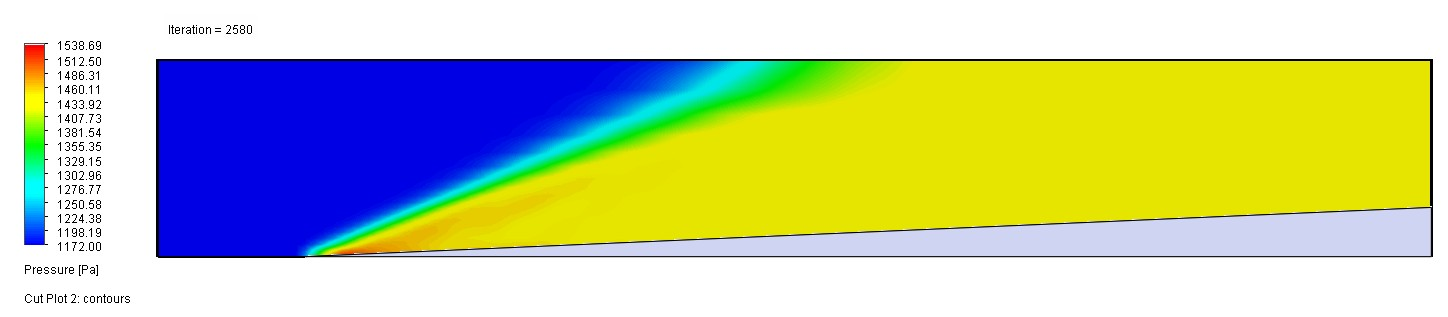
\includegraphics[width=0.8\linewidth]{ressources/images/CFD/SolidWorks2.jpg}
    \caption{SolidWorks pressure results}
    \label{fig:resSW}
\end{figure}

\subsubsection{Exportation}

To analyze the results algorithmically, we export the data from SolidWorks in \texttt{.txt} format and convert it to \texttt{.csv}. We ensure the header follows:
\begin{pycode}
lines[0] = 'X [m] Y [m] Z [m] Volume [m^3] Pressure [Pa]\n'
\end{pycode}

\subsection{Results analysis}

\subsubsection{\(1^{\text{st}}\) Visualization}

First, we verify the dataset and preview it in Python using Matplotlib to prepare for the pressure‐distribution plot.
\begin{figure}[H]
    \centering
    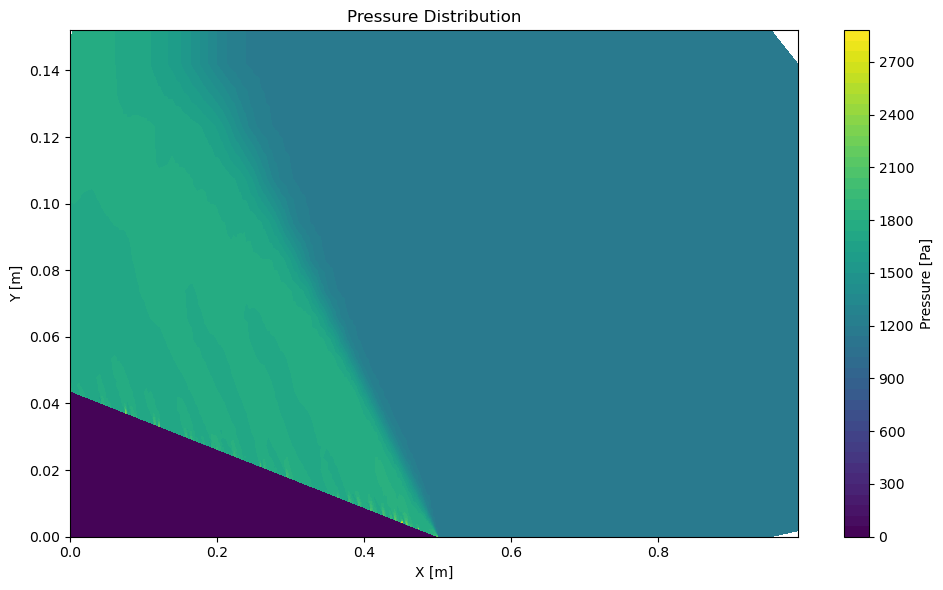
\includegraphics[width=0.5\linewidth]{ressources/figures/PressureDistribution.png}
    \caption{Initial visualization of pressure data}
    \label{fig:first_visualization}
\end{figure}
As expected, the dataset shows three pressure zones: upstream of the shock, downstream of the shock, and inside the solid region (where the pressure is zero).

\subsubsection{K-Means clustering}

We apply the unsupervised K-Means algorithm (\(k=3\)) to partition the data into the three zones (pre-shock, post-shock, solid interior). Once clustered, we extract the boundary points and plot them.
\begin{figure}[H]
    \centering
    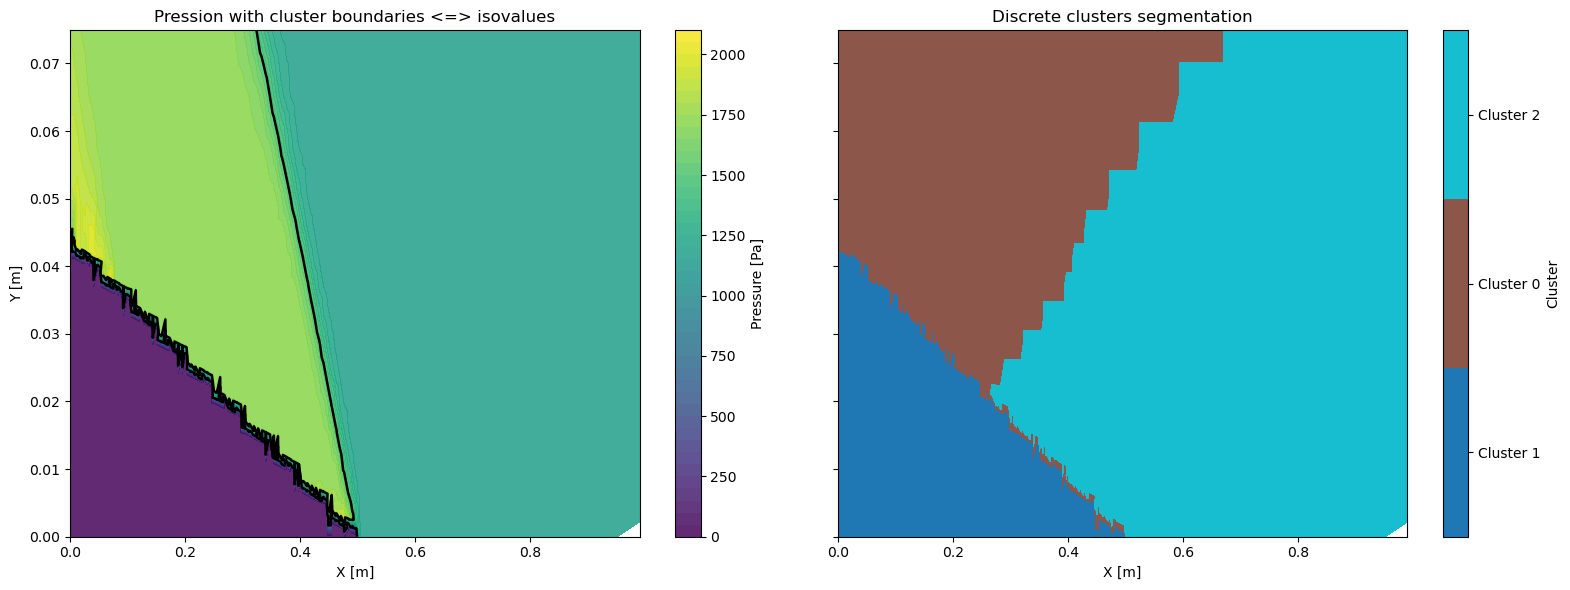
\includegraphics[width=0.8\linewidth]{ressources/figures/Kmeans.png}
    \caption{K-Means clustering of pressure zones}
    \label{fig:clustering}
\end{figure}

\subsubsection{Interpretation}

We perform linear fits on the boundary points to obtain slopes.
\begin{figure}[H]
    \centering
    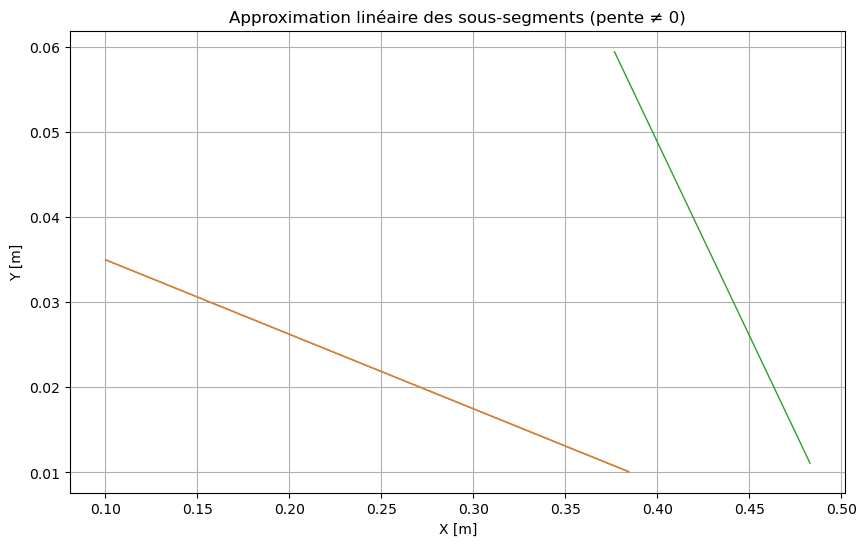
\includegraphics[width=0.5\linewidth]{ressources/figures/slope.png}
    \caption{Linear fits to boundary points}
    \label{fig:slopes}
\end{figure}
We discard the fits with the smallest variation, retaining only the shock boundary. From its slope we compute the shock angle, yielding:
\begin{figure}[H]
    \centering
    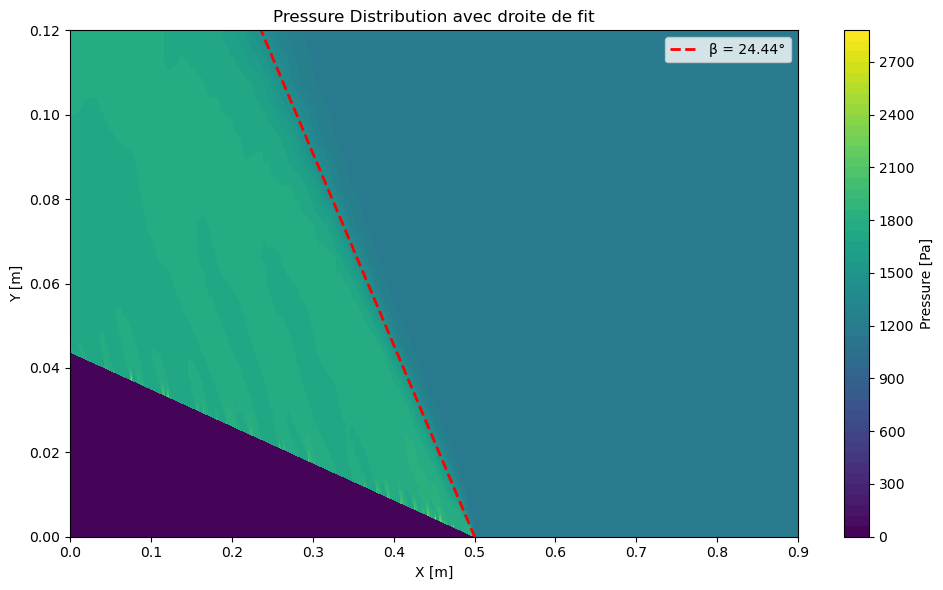
\includegraphics[width=0.5\linewidth]{ressources/figures/final_slope.png}
    \caption{Computed shock angle from slope}
    \label{fig:interpretation}
\end{figure}

\subsubsection{Repetition}

Using the same geometry and analysis procedure, we repeat the simulations to compare with theoretical values.
\begin{figure}[H]
    \centering
    \begin{minipage}[b]{0.45\linewidth}
        \centering
        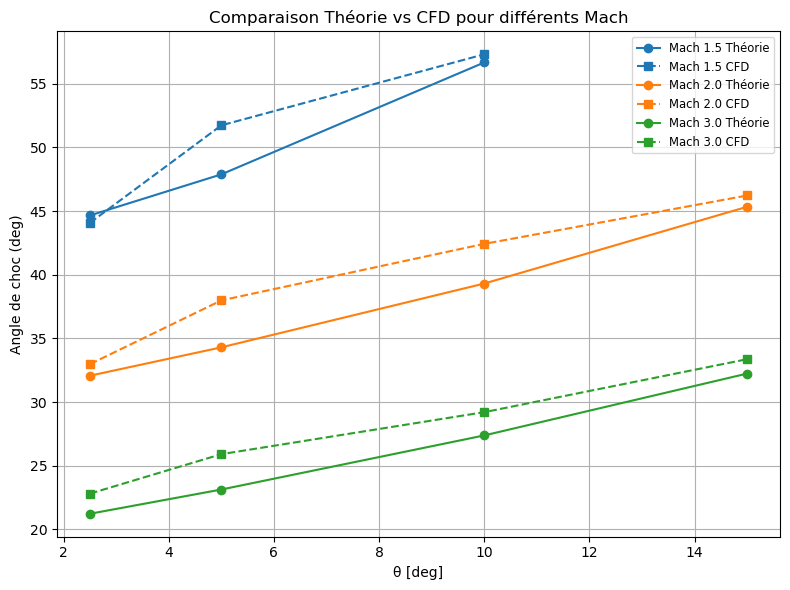
\includegraphics[width=\linewidth]{ressources/figures/sol1.png}
    \end{minipage}
    \hfill
    \begin{minipage}[b]{0.45\linewidth}
        \centering
        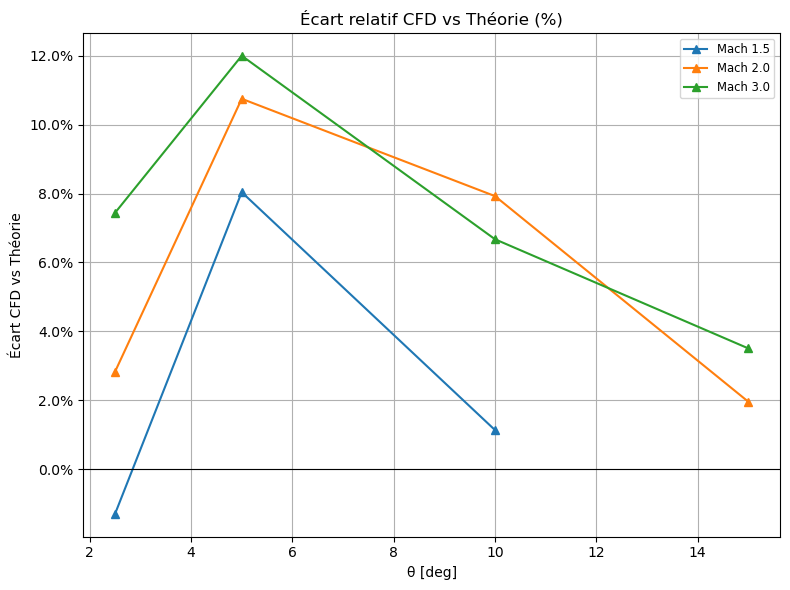
\includegraphics[width=\linewidth]{ressources/figures/sol2.png}
    \end{minipage}
    \caption{Comparison of simulation and theory}
    \label{fig:sol}
\end{figure}

Across all cases, the maximum deviation remains below 12 \%, demonstrating that the numerical results closely follow the theoretical predictions. The remaining discrepancy can be attributed chiefly to the theory’s assumption of infinitesimal thickness wich is not the case in reality and so in the CFD model.